\documentclass{article}
% translate with >> pdflatex -shell-escape <file>

\usepackage{pgfplots}
\pgfplotsset{compat=newest}

\pagestyle{empty}

\begin{document}
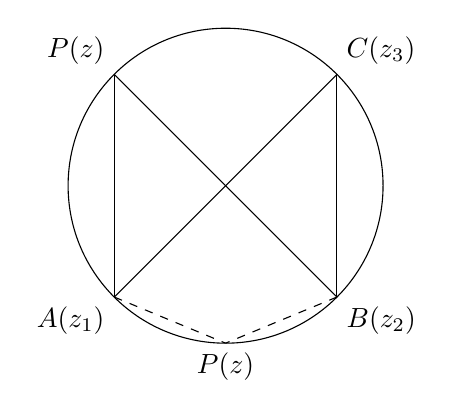
\begin{tikzpicture}%
   \draw (0,0) circle(2);
   \draw (1.414, -1.414) -- (1.414, 1.414);
   \draw (1.414, -1.414) -- (-1.414, 1.414);
   \draw[dashed] (1.414, -1.414) -- (0, -2);
   \draw (-1.414, -1.414) -- (1.414, 1.414);
   \draw (-1.414, -1.414) -- (-1.414, 1.414);
   \draw[dashed] (-1.414, -1.414) -- (0, -2);
   \draw (1.414, 1.414) node[anchor=south west] {$C(z_3)$};
   \draw (-1.414, 1.414) node[anchor=south east] {$P(z)$};
   \draw (-1.414, -1.414) node[anchor=north east] {$A(z_1)$};
   \draw (0, -2) node[anchor=north] {$P(z)$};
   \draw (1.414, -1.414) node[anchor=north west] {$B(z_2)$};
\end{tikzpicture}%
\end{document}

